\begin{minipage}[c]{\textwidth}
\advance\leftskip-2.5cm
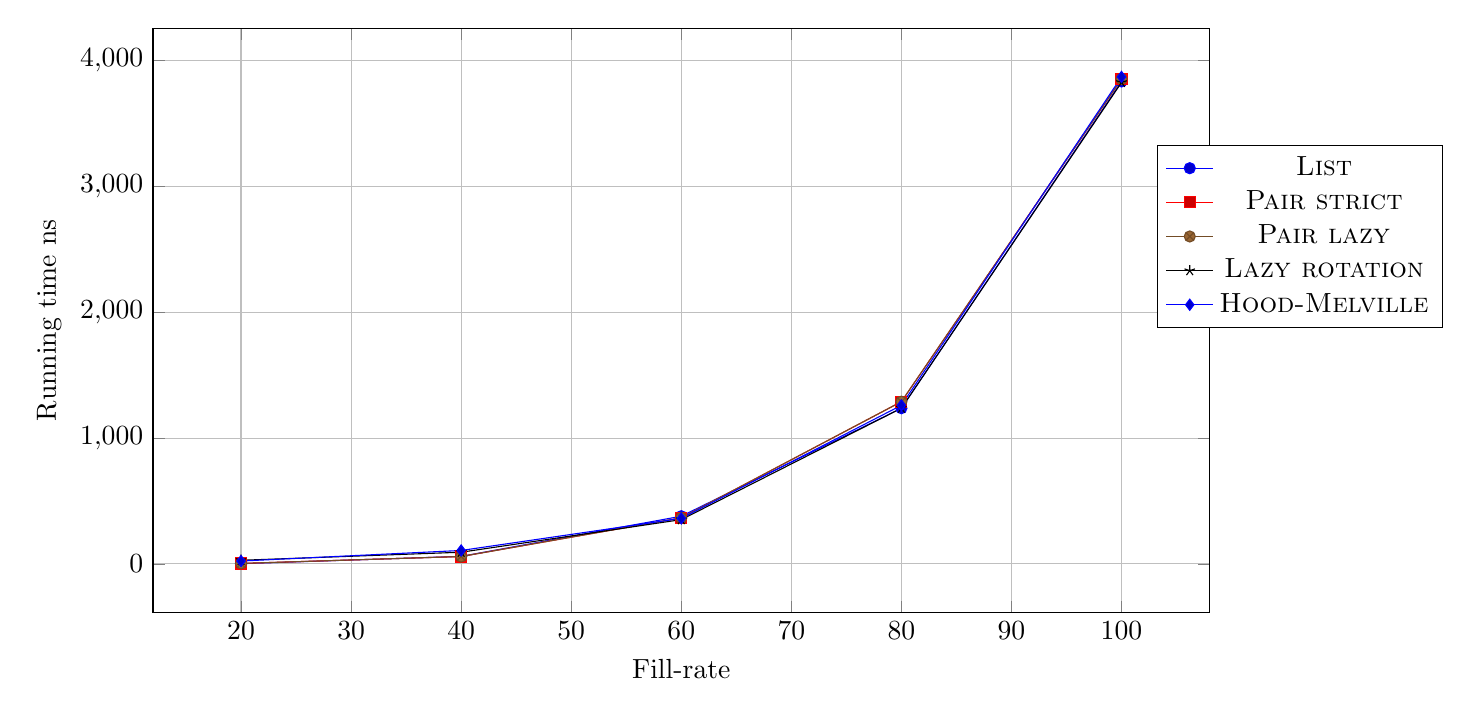
\begin{tikzpicture}
        \begin{axis}[
            xlabel = Fill-rate,
            ylabel = Running time ns,
            height=9cm,
            width=15cm,
            grid=major,
            legend style={
            at={(0.95,0.8)},
            anchor=north west}]            
            legend pos=center west
    	]
    		
    		
    	\addplot coordinates {
(20,2)
(40,60)
(60,379)
(80,1237)
(100,3833)

    	};
        
    	\addlegendentry{\textsc{List}}

                \addplot coordinates {
(20,4)
(40,59)
(60,366)
(80,1289)
(100,3852)

    	};
        
    	\addlegendentry{\textsc{Pair strict}}

        \addplot coordinates {
(20,4)
(40,59)
(60,366)
(80,1289)
(100,3852)

    	};
        
    	\addlegendentry{\textsc{Pair lazy}}

        \addplot coordinates {
(20,29)
(40,93)
(60,352)
(80,1237)
(100,3825)

    	};
        
    	\addlegendentry{\textsc{Lazy rotation}}

        \addplot coordinates {
(20,23)
(40,107)
(60,362)
(80,1260)
(100,3869)

    	};
        
    	\addlegendentry{\textsc{Hood-Melville}}

        \end{axis}

    \end{tikzpicture}
    \captionof{figure}{TITEL}
    \label{fig:sample_figure}
\end{minipage}